\documentclass{exam}

\input{preamble.sty}
\begin{document}
\begin{center}
    \Large
\textbf{Lab 6: Single-Qubit Trajectories}
\end{center}
    \section{Equator Tour}
    \subsection{Calculations}
    The flowing circuit is implemented, looking at the how the state vector changes on the Bloch sphere after initialization and each gate.
    \begin{center}
            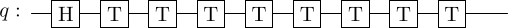
\includegraphics[width = .50 \linewidth]{images/Lab6_part1_circuit.png}
    \end{center}
    \begin{center}
        \begin{tabular}{|c|c|c|c|}
            \hline
            \textbf{Step} & \textbf{Bloch (x,y,z)} & \textbf{Angle from prev} & \textbf{Gate effect}\\ \hline
            $\ket{0}$ & (0,0,1) & --- & Start\\ \hline
            $\hat{H}$ & (1,0,0) & 90$^\circ$ (off $z$-axis)& Equator (On $+x$ axis)\\ \hline
            $\hat{T}$ & ($\frac{1}{\sqrt{2}}$,$\frac{1}{\sqrt{2}}$,0) & 45$^\circ$ (off $x$-axis) & Half way between $+x$ and $+y$\\ \hline
            $\hat{T}$ & (0,1,0) & 45$^\circ$ (off $x$-axis) & On $+y$ axis \\ \hline
            $\hat{T}$ & (-$\frac{1}{\sqrt{2}}$,$\frac{1}{\sqrt{2}}$,0) & 45$^\circ$ (off $x$-axis) & Half way between $-x$ and $+y$\\ \hline
            $\hat{T}$ & (-1,0,0) & 45$^\circ$ (off $x$-axis) & On $-x$ axis\\ \hline
            $\hat{T}$ & (-$\frac{1}{\sqrt{2}}$,-$\frac{1}{\sqrt{2}}$,0) & 45$^\circ$ (off $x$-axis) & Half way between $-x$ and $-y$\\ \hline
            $\hat{T}$ & (0,-1,0) & 45$^\circ$ (off $x$-axis) & On $-y$ axis\\ \hline
            $\hat{T}$ & ($\frac{1}{\sqrt{2}}$,-$\frac{1}{\sqrt{2}}$,0) & 45$^\circ$ (off $x$-axis) & Half way between $+x$ and $-y$\\ \hline
            $\hat{T}$ & (1,0,0) & 45$^\circ$ (off $x$-axis) & On $+x$ axis\\ \hline
            \textbf{Total Path} & \multicolumn{2}{|c|}{90$^\circ$ (off $z$-axis), 360$^\circ$ (around $z$-axis)}& $\ket{+}$\\ \hline
        \end{tabular}
    \end{center}
    This makes a counter-clockwise rotation (from the view of the Bloch Sphere Plot) starting and ending on the positive $x$-axis.\\
            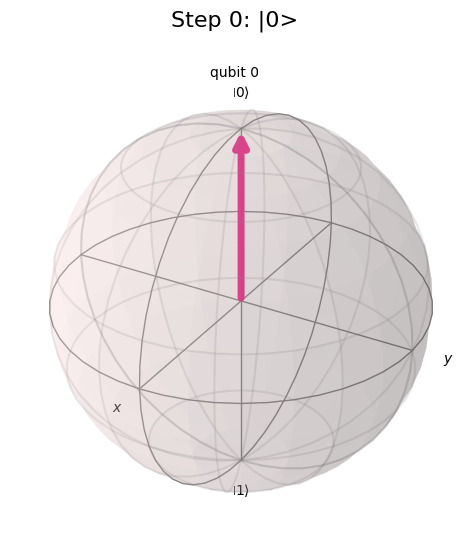
\includegraphics[width = .20 \linewidth]{images/Lab6_part1_bloch_1.png}
            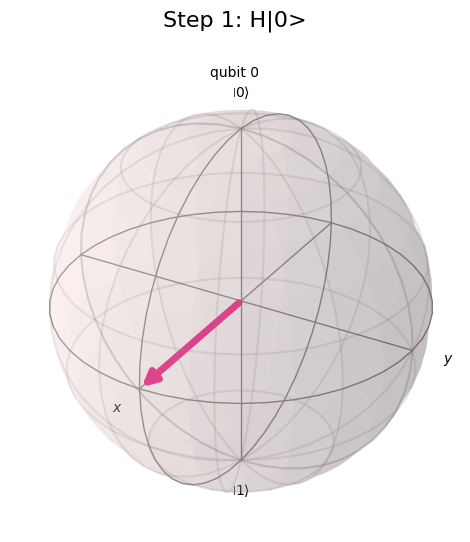
\includegraphics[width = .20 \linewidth]{images/Lab6_part1_bloch_2.png}
            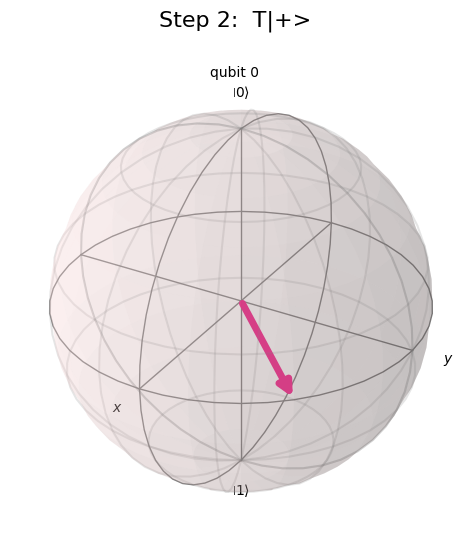
\includegraphics[width = .20 \linewidth]{images/Lab6_part1_bloch_3.png}
            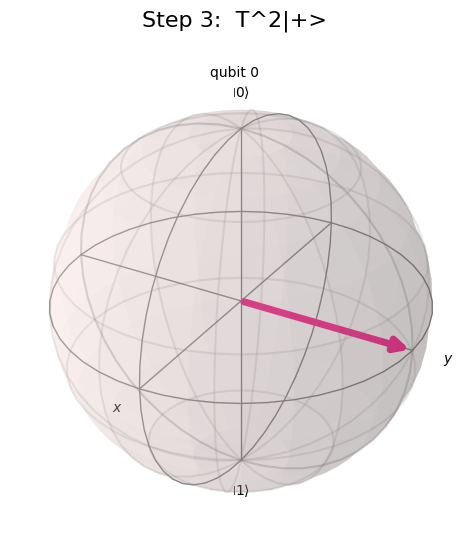
\includegraphics[width = .20 \linewidth]{images/Lab6_part1_bloch_4.png}
            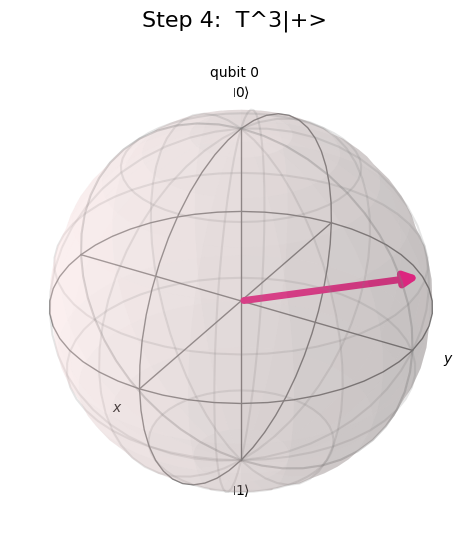
\includegraphics[width = .20 \linewidth]{images/Lab6_part1_bloch_5.png}
            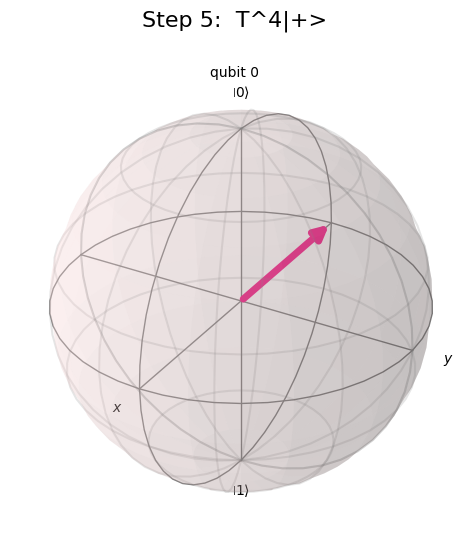
\includegraphics[width = .20 \linewidth]{images/Lab6_part1_bloch_6.png}
            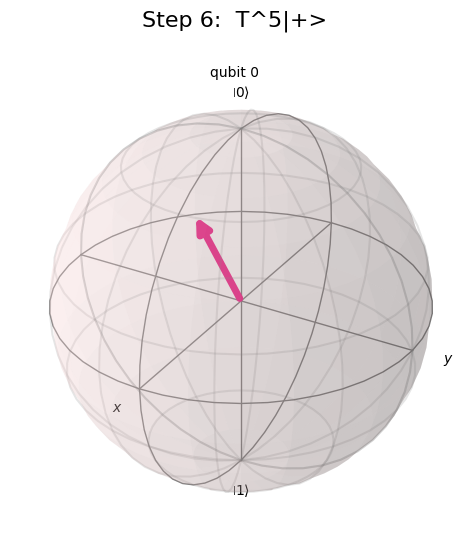
\includegraphics[width = .20 \linewidth]{images/Lab6_part1_bloch_7.png}
            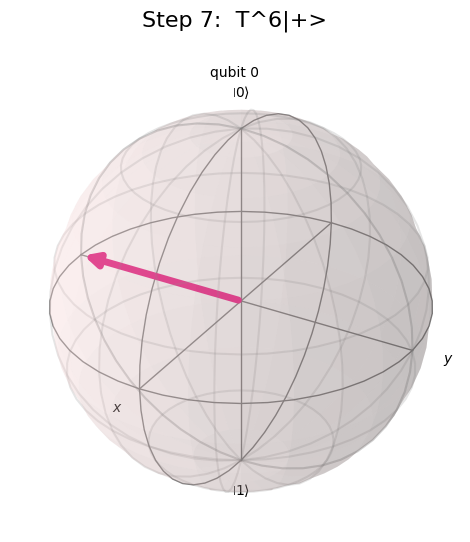
\includegraphics[width = .20 \linewidth]{images/Lab6_part1_bloch_8.png}
            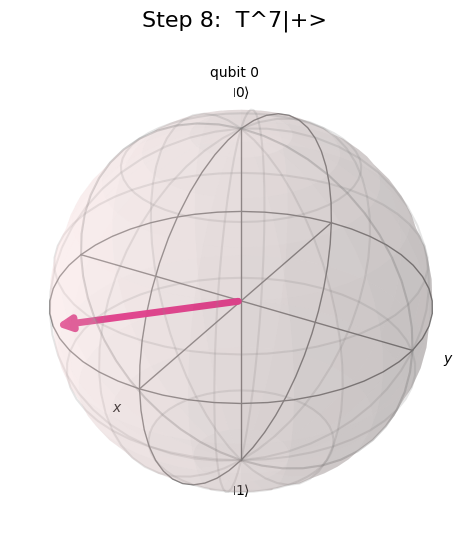
\includegraphics[width = .20 \linewidth]{images/Lab6_part1_bloch_9.png}
            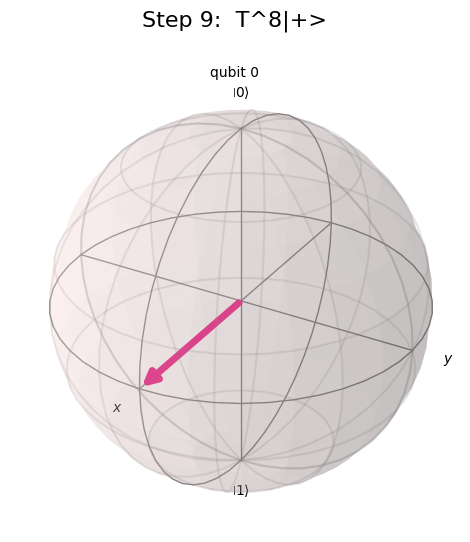
\includegraphics[width = .20 \linewidth]{images/Lab6_part1_bloch_10.png}
    
    \subsection{Code}
    \begin{verbatim}
        qc = [0,0,0,0,0,0,0,0,0,0]
        state = [0,0,0,0,0,0,0,0,0,0]

        qc[0] = QuantumCircuit(1)
        state[0] = Statevector(qc[0])
        plot_bloch_multivector(state[0], title="Step 0: |0>")
        qc[1] = qc[0].copy()
        qc[1].h(0)
        state[1] = Statevector(qc[1])
        plot_bloch_multivector(state[1], title="Step 1: H|0>")
        for i in range(2,10):
            qc[i] = qc[i-1].copy()
            qc[i].t(0)
            state[i] = Statevector(qc[i])
            if i==2:
                plot_bloch_multivector(state[i], title=f"Step {i}:  T|+>")
            else:
                plot_bloch_multivector(state[i], title=f"Step {i}:  T^{i-1}|+>")
    \end{verbatim}

    \section{Pauli Ladder}
    \subsection{Calculations}
    The flowing circuit is implemented, looking at the how the state vector changes on the Bloch sphere after initialization and each gate.
    \begin{center}
            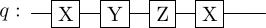
\includegraphics[width = .25 \linewidth]{images/Lab6_part2_circuit.png}
    \end{center}
    \begin{center}
        \begin{tabular}{|c|c|c|c|}
            \hline
            \textbf{Step} & \textbf{Bloch (x,y,z)} & \textbf{Angle from prev} & \textbf{Gate effect}\\ \hline
            $\ket{0}$ & (0,0,1) & --- & Start\\ \hline
            $\hat{X}$ & (0,0,-1) & 90$^\circ$ (off $z$-axis)& Equator (On $+x$ axis)\\ \hline
            $\hat{Y}$ & (0,0,1) & 45$^\circ$ (off $x$-axis) & Half way between $+x$ and $+y$\\ \hline
            $\hat{Z}$ & (0,0,1) & 45$^\circ$ (off $x$-axis) & On $+y$ axis \\ \hline
            $\hat{X}$ & (0,0,-1) & 45$^\circ$ (off $x$-axis) & Half way between $-x$ and $+y$\\ \hline
            \textbf{Total Path} & \multicolumn{2}{|c|}{180$^\circ$ (off $z$-axis)}& $\ket{1}$\\ \hline
        \end{tabular}
    \end{center}
    This flips the vector switching between pointing up ($\ket{0}$) to down ($\ket{1}$) in the pattern: Up, Down, Up, Up, Down.\\
            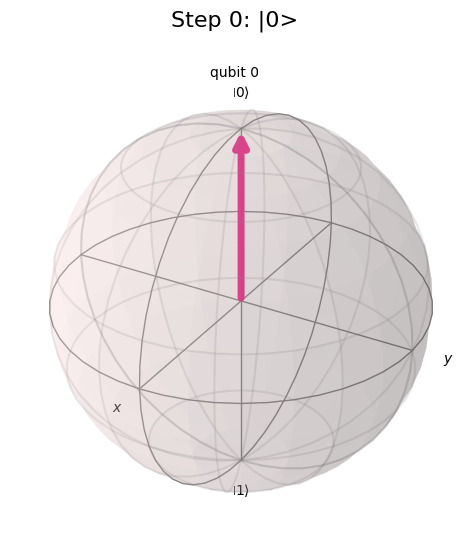
\includegraphics[width = .20 \linewidth]{images/Lab6_part2_bloch_1.png}
            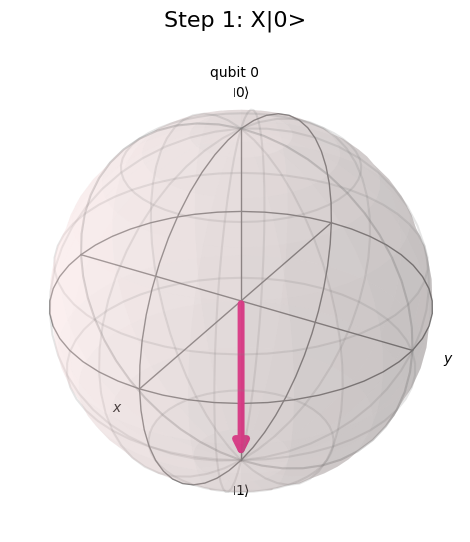
\includegraphics[width = .20 \linewidth]{images/Lab6_part2_bloch_2.png}
            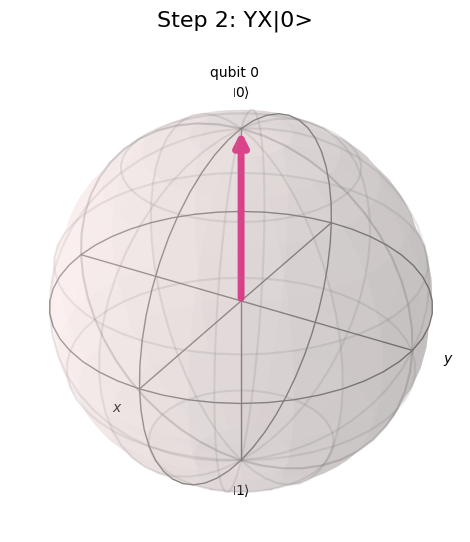
\includegraphics[width = .20 \linewidth]{images/Lab6_part2_bloch_3.png}
            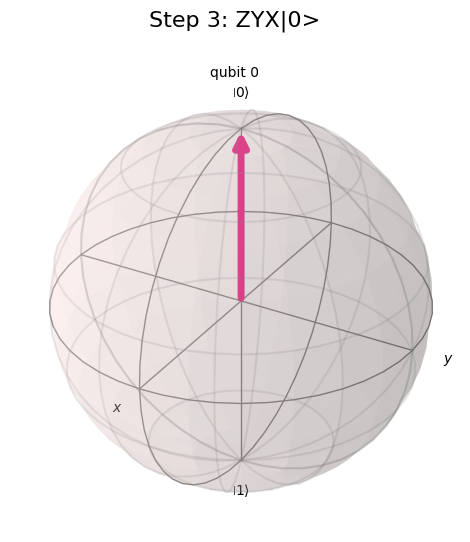
\includegraphics[width = .20 \linewidth]{images/Lab6_part2_bloch_4.png}
            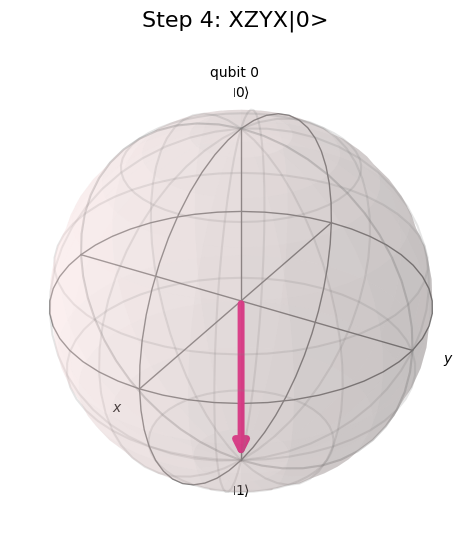
\includegraphics[width = .20 \linewidth]{images/Lab6_part2_bloch_5.png}
    
    \subsection{Code}
    \begin{verbatim}
        qc_2 = [0,0,0,0,0]
        state_2 = [0,0,0,0,0]

        qc_2[0] = QuantumCircuit(1)
        state_2[0] = Statevector(qc_2[0])
        plot_bloch_multivector(state_2[0], title="Step 0: |0>")

        qc_2[1] = qc_2[0].copy()
        qc_2[1].x(0)
        state_2[1] = Statevector(qc_2[1])
        plot_bloch_multivector(state_2[1], title="Step 1: X|0>")

        qc_2[2] = qc_2[1].copy()
        qc_2[2].y(0)
        state_2[2] = Statevector(qc_2[2])
        plot_bloch_multivector(state_2[2], title="Step 2: YX|0>")

        qc_2[3] = qc_2[2].copy()
        qc_2[3].z(0)
        state_2[3] = Statevector(qc_2[2])
        plot_bloch_multivector(state_2[2], title="Step 3: ZYX|0>")

        qc_2[4] = qc_2[3].copy()
        qc_2[4].x(0)
        state_2[4] = Statevector(qc_2[4])
        plot_bloch_multivector(state_2[4], title="Step 4: XZYX|0>")
    \end{verbatim}

       \section{Pauli Ladder}
    \subsection{Calculations}
    The flowing circuit is implemented, looking at the how the state vector changes on the Bloch sphere after initialization and each gate.
    \begin{center}
            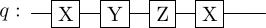
\includegraphics[width = .25 \linewidth]{images/Lab6_part2_circuit.png}
    \end{center}
    \begin{center}
        \begin{tabular}{|c|c|c|c|}
            \hline
            \textbf{Step} & \textbf{Bloch (x,y,z)} & \textbf{Angle from prev} & \textbf{Gate effect}\\ \hline
            $\ket{0}$ & (0,0,1) & --- & Start\\ \hline
            $\hat{X}$ & (0,0,-1) & 90$^\circ$ (off $z$-axis)& Equator (On $+x$ axis)\\ \hline
            $\hat{Y}$ & (0,0,1) & 45$^\circ$ (off $x$-axis) & Half way between $+x$ and $+y$\\ \hline
            $\hat{Z}$ & (0,0,1) & 45$^\circ$ (off $x$-axis) & On $+y$ axis \\ \hline
            $\hat{X}$ & (0,0,-1) & 45$^\circ$ (off $x$-axis) & Half way between $-x$ and $+y$\\ \hline
            \textbf{Total Path} & \multicolumn{2}{|c|}{180$^\circ$ (off $z$-axis)}& $\ket{1}$\\ \hline
        \end{tabular}
    \end{center}
    This flips the vector switching between pointing up ($\ket{0}$) to down ($\ket{1}$) in the pattern: Up, Down, Up, Up, Down.\\
            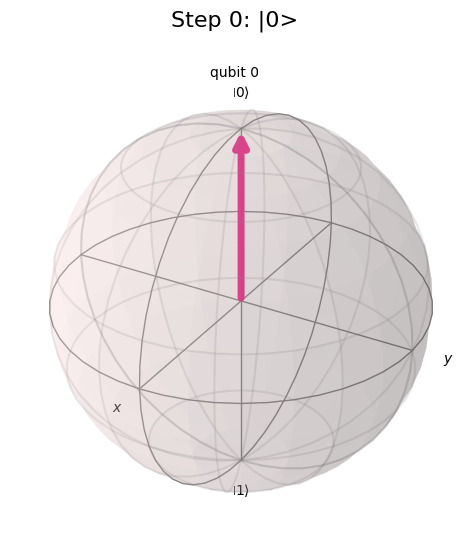
\includegraphics[width = .20 \linewidth]{images/Lab6_part2_bloch_1.png}
            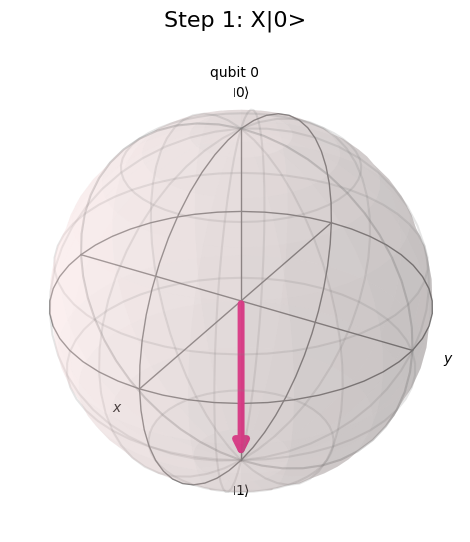
\includegraphics[width = .20 \linewidth]{images/Lab6_part2_bloch_2.png}
            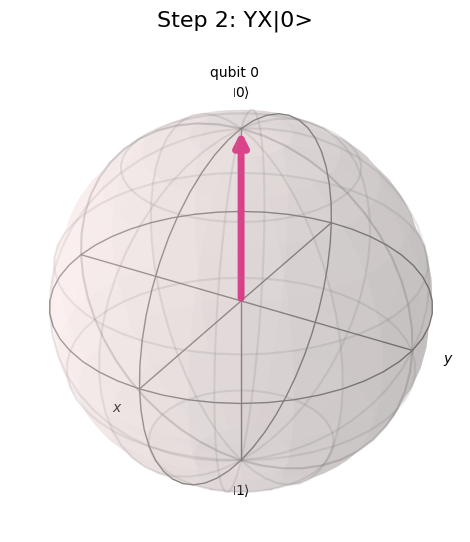
\includegraphics[width = .20 \linewidth]{images/Lab6_part2_bloch_3.png}
            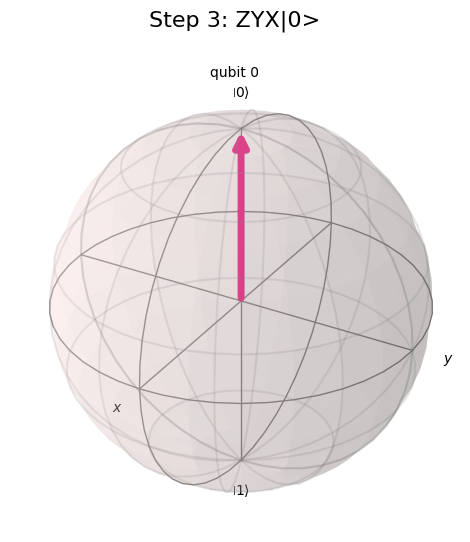
\includegraphics[width = .20 \linewidth]{images/Lab6_part2_bloch_4.png}
            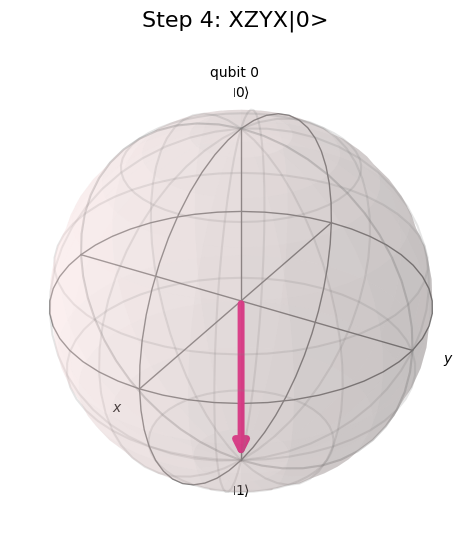
\includegraphics[width = .20 \linewidth]{images/Lab6_part2_bloch_5.png}
    
    \subsection{Code}
    \begin{verbatim}
       
    \end{verbatim}
    
\end{document}